\documentclass[a4paper, 11pt]{article}

\voffset -0cm
\hoffset 0.0cm
\textheight 23cm
\textwidth 16cm
\topmargin 0.0cm
\oddsidemargin 0.0cm
\evensidemargin 0.0cm

\usepackage[ruled,vlined,linesnumbered]{algorithm2e}   % authors: last version of algorithm display

\usepackage{epsfig}
\usepackage{setspace}
\usepackage{fancyheadings}
\usepackage{amsmath}
\usepackage{amssymb}
\usepackage{graphicx}
\usepackage{url}
\newtheorem{Lemma}{Lemma}

\title{}
\author{}
\date{}

\newtheorem{qu}{Question}

\begin{document}

\begin{center}
	\LARGE \textbf{TD: ``Images et g\'eom\'etrie discr\`ete''\\Extended Euclid's Algorithm}
\end{center}


Let us consider the following Euclidean division algorithm.

\begin{procedure}[H]
\caption{Convergents( $\text{(a,b), (p,q), (p',q'), i}$ )}
\label{algo:conv}
\KwIn{$(a,b)$, $(p,q)$, $(p',q')$, $i$}
\KwOut{$(p',q')$}
%
Let $r$ be the remainder of the Euclidean division $b/a$\;
Let $u$ be the quotient  of the Euclidean division $b/a$\;
$p'' \leftarrow up' + p$\; $q'' \leftarrow uq' + q$\;
\eIf{$r > 0$}{
 \Return{Convergents($(r,a)$, $(p',q')$, $(p'',q''), i+1$)}\;
}{
 \Return{$(p',q')$}
}
\end{procedure}


\begin{qu}
\label{qu:init}
  Let $(p_{-1},q_{-1})=(1,0)$ and $(p_0,q_0)=(0,1)$, what is the
  output of \emph{\texttt{Convergents}}($(5,8)$, $(p_{-1},q_{-1})$,
  $(p_0,q_0)$, 0) ?
\end{qu}


\begin{qu}
  Let us consider \emph{\texttt{Convergents}}($(a,b)$, $(p_{-1},q_{-1})$,
  $(p_0,q_0)$, 0) (with $0 \leq a < b$ and $\gcd{(a,b)} = 1$). We
  index the recursive calls by $i=1\ldots n$. Show that
  \begin{displaymath}
    \forall i=1\ldots n\,, p_i=u_ip_{i-1}+p_{i-2}\text{ and } q_i=u_iq_{i-1}+q_{i-2}\,.
  \end{displaymath}
\end{qu}


\begin{qu}
Similarly, with $r_{-1}=b$ and $r_0=a$, show that
  \begin{displaymath}
    \forall i=1\ldots n\,, r_i=r_{i-2}- u_ir_{i-1}
  \end{displaymath}
\end{qu}

\begin{qu}
  Following previous results, prove the following statements:

  \begin{enumerate}
  \item $\forall i=1\ldots n\,, p_{i-1}q_i - q_{i-1}p_i = \pm 1$
  \item $\forall i=-1\ldots n\,, p_{i}b - q_{i}a = \pm r_i$
  \end{enumerate}
Since $r_n=gcd(a,b)=1$, what is $p_nb-q_na$ ?
\end{qu}

\begin{qu}Give the definition of uni-modularity. What is the
  geometrical interpretation of this definition ?
\end{qu}


\begin{qu}
  In the domain in appendix, draw the Euclidean segment
  $[(0,0)-(b,a)]$ and all convergents $(q_i,p_i)$ for the input given
  in Question \ref{qu:init}. With respect to the parity of $i$, can
  you say something on the position of convergents with respect to the
  segment ? If we construct a polygonal curve with only convergents
  $(q_i,p_i)$ with even index $i$ (plus a last point $(b,a)$). What
  kind of geometrical object I have constructed ?
\end{qu}


\begin{qu}
  Let $L_{odd}$ (resp. $L_{even}$) be the polygonal curve of convergents with
  odd index (resp. even index). Furthermore, we add the point $(b,a)$
  to the end of each list. For the input given in Question
  \ref{qu:init}, are there integer points between $L_{odd}$ and
  $L_{even}$ ? Why ?
\end{qu}


\begin{qu}
  For a general setting \emph{\texttt{Convergents}}($(a,b)$, $(p_{-1},q_{-1})$,
  $(p_0,q_0)$, 0), can you prove the statement of the previous
  question ?
\end{qu}

\begin{qu}
  What is the complexity of \emph{\texttt{Convergents}} with respect
  to $a$ and $b$ ?
\end{qu}





\newpage
\appendix

\begin{center}
  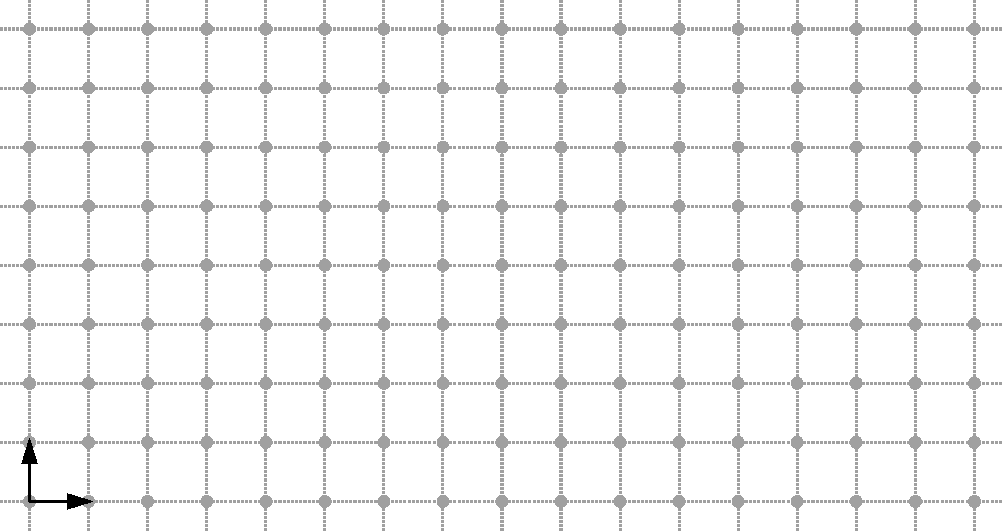
\includegraphics[width=8cm]{domain}
\end{center}


\begin{center}
  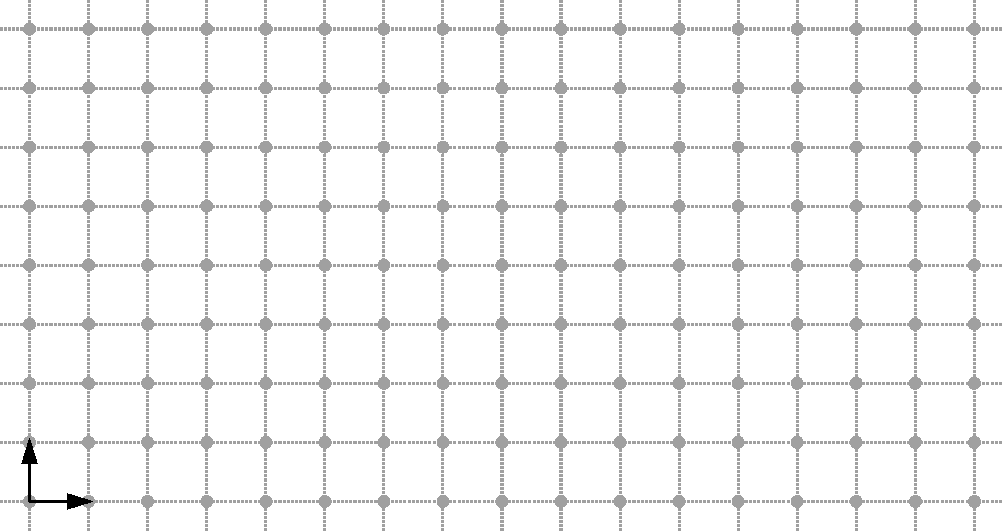
\includegraphics[width=8cm]{domain}
\end{center}


\end{document}
